%
% Documento: Disposições
%

\chapter{Framework Proposto}

    Neste capítulo irei abordar as tecnologias de utilizadas para a codificação do framework,
    detalhando os modulos e suas classes expostas para o usuario e as ferramentas utilizadas
    para controle de versão e publicação do framework.


    \section{Tecnologias Utilizadas}

        Para o desenvolvimento do framework foi utilizado apenas como linguagem para desenvolvimento o Python
        e para a manipulação e integração com o browser a biblioteca em python do Selenium Webdriver. Por ser um
        projeto que visa ser o mais simples e leve possivel apenas os modulos padrões do python estão sendo utilizado
        para o desenvolvimento desta ferramenta.


        \subsection{Python}

            A escolha do Python \cite{python} foi devida porque ele trata-se de uma linguagem de programação fácil de aprender e poderosa.
            Possuindo uma estruturas dados de alto nível e uma abordagem simples, mas eficaz, para a programação orientada
            a objetos. Contendo uma Sintaxe elegante e tipagem dinâmica, juntamente com uma interpretação natural, tornam
            a linguagem ideal para criação dos scripts do pybot.

        \subsection{Selenium WebDriver}
            Selenium Webdriver \cite{webdriver} é um framework utilizado para se comunicar e enviar comandos para os browser
            em conjunto com um controlador de cada browser especifico. Em comparação com seu antecessor, Selenium RC, o Selenium Webdriver
            não precisa de um server para enviar os comandos para o browser. Utilizando comando nativos do sistema operacional ao invés de
            comando javascript, usados pelo Selenium RC, deixam o Selenium Webdriver uma excelente ferramenta para integração com diversos
            browser.

        \subsection{Git e GitHub}
            Para o controle de versões e alterações do codigo fonte do framework e scripts de exemplo foi utilizado a ferramenta
            Git \cite{git} em conjunto com os servidores do Github \cite{github} para hospedagem e gerenciamento. Com eles foi possivel
            fazer alterações dos codigos fontes em qualquer computador e gerenciar os erros e melhorias do framework.


    \section{Modulos}

        O framework consiste em alguns modulos basicos, cada um com suas devidas utilidades e funções.
        A separação dos de cada modulos foi dada com base em suas caracteristicas e funcionalidades,

        \begin{figure}[H]
            \vspace*{0,3cm}
            \centering
            \caption{Diagrama de Componentes}
            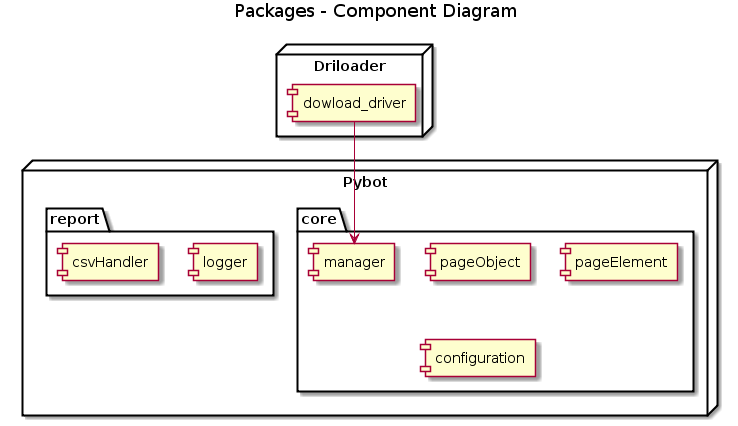
\includegraphics[width=1\textwidth]{./04-figuras/model}
            \label{fig:modules}
        \end{figure}

        \subsection{Core}
            Este modulo contem as funcionalidades basicas para a operação do framework com o Selenium Webdriver
            e o gerenciamento dos parâmetros de execuções de cada script.

            \subsubsection{Manager}
            Manager server para abstrair o uso do Selenium Webdriver criando uma camada de metodos propios fazendo com que caso alguma
            atualiação da API do Selenium Webdriver altere os scripts criados não sejam impactados. Fazendo uso do Driloader mencionado na
            subseção \ref{driloader} ele verifica a necessidade do download do driver para poder executar o Selenium Webdriver.

            \subsubsection{Configuration}
            Responsavel por gerar as configurações basicas para o framework e disponibiliza-las no arquivo \emph{pybot.ini}.
            Este arquivo é criado para cada script do usuario e nele arquivo é possivel adicionar quaisquer tipo de configurações ou parâmetros
            necessarias para o usuario, apenas sendo necessario seguir os padrões descrito na imagem \ref{fig:pybot.ini} e utilizando com o comando
            \mbox{\emph{configuration.getConfig('Seção', 'variavel')}}

            \begin{figure}[H]
                \vspace*{0,3cm}
                \centering
                \caption{Estrutura pybot.ini}
                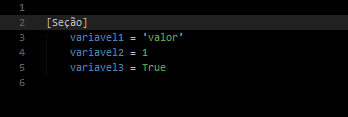
\includegraphics[width=0.7\textwidth]{./04-figuras/ini}
                \label{fig:pybot.ini}
            \end{figure}

        \subsection{Component}
        \label{Comp}
            Modulo criado para seguir os padrões de \emph{PageObject} e \emph{PageElement}, contendo abstração para os tipos de inputs do html.

            \subsubsection{WebElement}
                Serve para abstrair o uso da classe WebElement do proprio Selenium Webdriver. Contendo uma classe para cada tipo de campo dos html,
                ele dispõe de algumas funcionalidades basica, como a atribuição de uma valor para um elemento do tipo \emph{input text} irá excrever
                valor dentro do campo, \emph{select} irá selecionar a opção cujo texto seja igual ao valor informado, \emph{radio} irá selecionar o
                a opção que tenha o \emph{value} do valor informado e para o tipo \emph{checkbox} irá marcar ou desmarcar as opções se o valor for
                verdadeiro(True) ou falso(False)

            \subsubsection{PageElement e PageElements}
            \label{PageElement}
                Essas classes servem para controlar os elementos mapeados das telas. Sempre quando serão acessadas a classe faz novamente a pesquisa
                do elemento em tela, previnindo assim uma das excessões mais comum do Selenium Webdriver que é a \emph{StaleElementReferenceException},
                que é quando o elemento em questão não existe mais no DOM ou a referencia que tinha não é mais a mesma. Conta com uma lista de seletores
                que facilitam para o usuario buscar os elementos e deixam o codigo mais legivel. Usa-se a classe PageElements quando quiser pegar mais
                de um elemento com o mesmo seletor.

                \begin{figure}[H]
                    \vspace*{0,3cm}
                    \centering
                    \caption{Lista de Seletores}
                    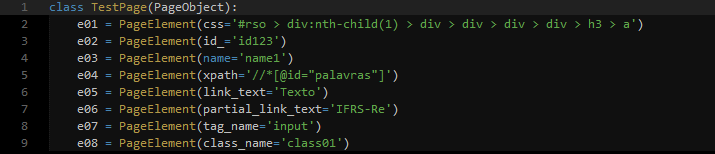
\includegraphics[width=1\textwidth]{./04-figuras/selectors}
                    \label{fig:selectors.png}
                \end{figure}

            \subsubsection{PageObject}
                Classe simbolica, serve apenas para poder juntar diversos PageElement descritos pelo usuario em uma classe para melhor
                legibilidade e componentização das paginas mapeadas.

        \subsection{Report}

            Estes modulo está destinado para geração de logs de execuções internas do framework, criação e controle
            de logs definidos pelos usuario e a criação de planilhas análiticas de dados extraidos das paginas.

            \subsubsection{Logger}
            Classe de geração dos Logs de execução do framework.

            \subsubsection{CsvHandler}
            Utilizado para geração de planilhas com dados extraidos das paginas para análise posterior do usuario.

        \subsection{Driloader}
        \label{driloader}
            Driloader é o responsavel pelo download dos driver de cada browser,suportanto download dos driver do Internet Explorer,
            Firefox e Chrome, sendo possivel para o usuario selecionar uma versão especifica, a ultima versão ou detectar
            automaticamente qual a versão adequada para o browser instalado do usuario. Como para utilizar do Selenium
            Webdriver é necessario um driver especifico de cada browser foi tomada a decisão da criação desse projeto,
            inicialmente o Driloader era um modulo do framework mas pela autonomia e praticidade que ele proporciona aos
            usuarios do Selenium Webdriver foi feita a separação dele do pybot.



